
\fullcite{zhpw03}

see also zhwa13.

\begin{multicols}{2}
\begin{center}
{\bf Article excerpts}
\\ 
{\bf Notes and remarks}
\end{center}
\end{multicols}

\begin{multicols}{2}
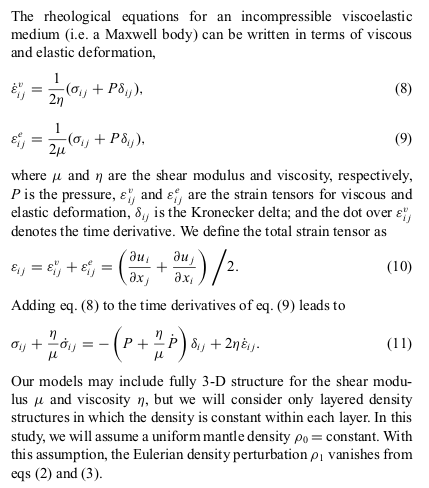
\includegraphics[width=8cm]{images/viscoelasticity/zhpw03_a}\\
\[
{\bm \sigma} =-p {\bm 1} + 2\eta \dot{\bm\varepsilon}_{\rm v}
\Rightarrow
\dot{\bm\varepsilon}_{\rm v} = \frac{1}{2\eta} ({\bm \sigma} + p {\bm 1})
\]
\[
{\bm \sigma} =-p {\bm 1} + 2\mu {\bm\varepsilon}_{\rm e}
\Rightarrow
{\bm\varepsilon}_{\rm e} = \frac{1}{2\mu} ({\bm \sigma} + p {\bm 1})
\]
\begin{eqnarray}
\dot{\bm\varepsilon}
&=& \dot{\bm\varepsilon}_{\rm v}+\dot{\bm\varepsilon}_{\rm e} \nn\\
&=& \frac{1}{2\eta} ({\bm \sigma} + p {\bm 1}) 
+ \frac{1}{2\mu} (\dot{\bm \sigma} + \dot{p} {\bm 1}) 
\end{eqnarray}

This leads to
\[
{\bm \sigma} + \frac{\eta}{\mu} \dot {\bm \sigma} = 
-\left(p + \frac{\eta}{\mu} \dot{p}\right) {\bm 1} + 2 \eta  \dot{\bm\varepsilon}
\]
\end{multicols}

\begin{multicols}{2}
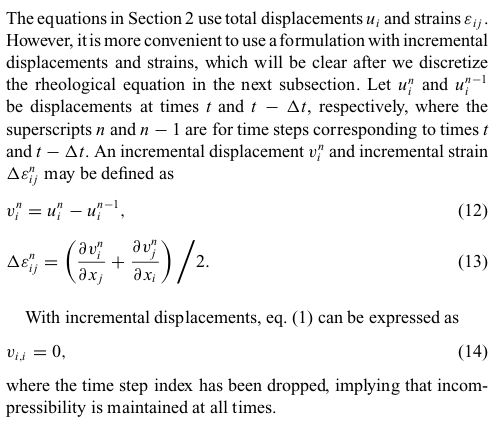
\includegraphics[width=8cm]{images/viscoelasticity/zhpw03_b}\\
\end{multicols}

\newpage

\begin{multicols}{2}
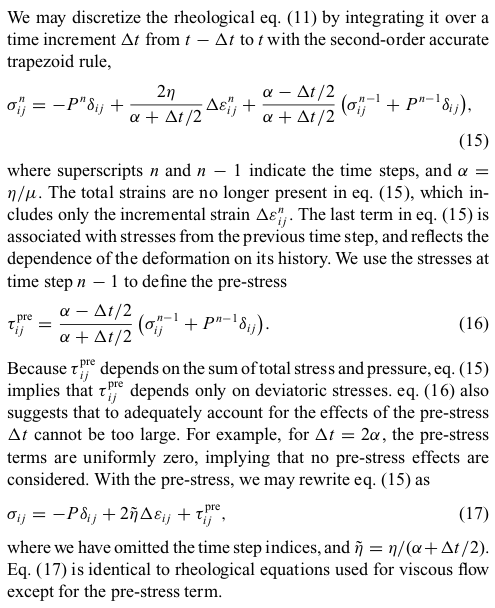
\includegraphics[width=8cm]{images/viscoelasticity/zhpw03_c}\\
\end{multicols}
